%!TEX root = ../dissertation.tex
\begin{savequote}[75mm]
Language is a process of free creation; its laws and principles are fixed, but the manner in which the principles of generation are used is free and infinitely varied.
\qauthor{Noam Chomsky}
\end{savequote}

\chapter{Dynamic Multimodal Network}

\newthought{On this chapter, a new model to handle language and vision features to define a segmentation mask is proposed}, by merging previous ideas and insights (as they were described on Chapter \ref{chap:previous_work}) with state-of-the art models in both visual and language recognition tasks. This model shall take the name of Dynamic Multimodal Network (DMN), as it not only processes language and visual information in a recurrent fashion \cite{li2017cvpr} (Multimodal Network) by taking visual and language information as a concatenated entity \cite{hu2016segmentation}, but it also generates and applies a set of dynamic filters based on the language representation to the visual one at each time step, inspired on \cite{liu2017segmentation}. Additionally, a new sampling module is proposed, based on the effectiveness of skip connections \cite{DBLP:journals/corr/RonnebergerFB15} to refine and produce segmentations masks that fit each object contour accordingly.

As shown on Figure~\ref{Fig:Overall} The DMN consists of four modules

\begin{figure}
\centering
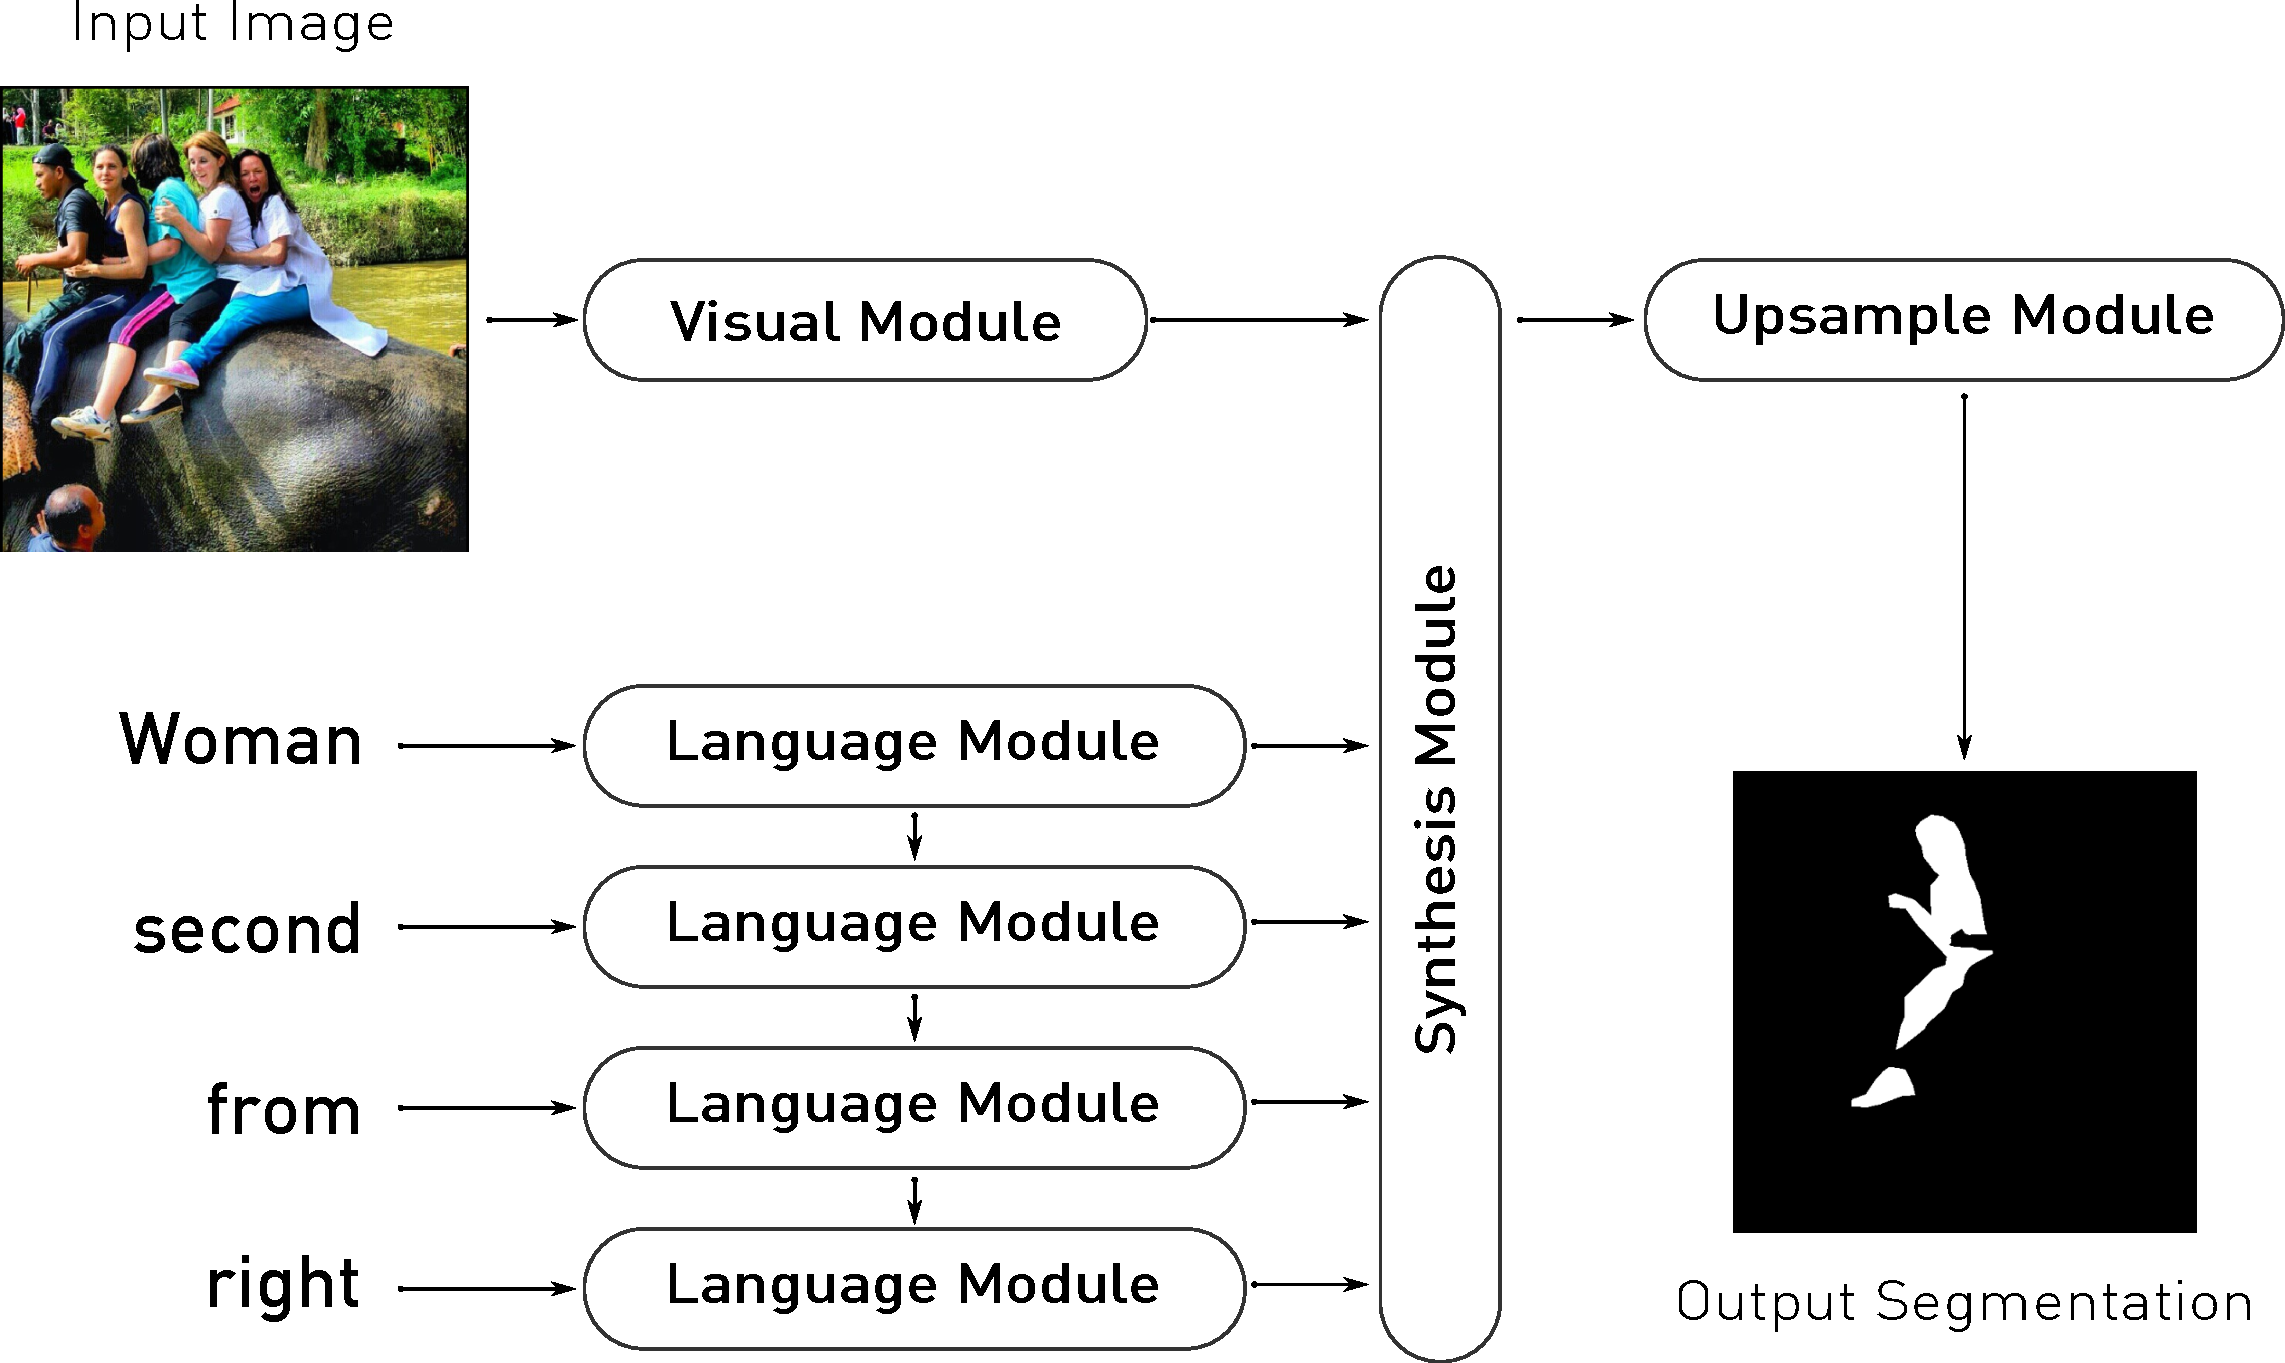
\includegraphics[width=\textwidth]{./figures/Model_Overview.pdf}
\caption{Dynamic Multimodal Network general overview consisting of a Visual Module, a Language Module, a Synthetic Module and a Upsampling Module}
\label{Fig:Overall}
\end{figure}
